\section{Architecture}

\subsection{Noyau}
\begin{frame}{Architecture}{Noyau}
	Le noyau Linux est un binaire de type ELF.\\
	Son image est souvent compréssé pour gagner en taille lors du déploiement et de la copie en RAM\\
	Il contient un auto extracteur qui va le décomprésser\\
	Fournit des services nécéssaires à sa fonction:
	\begin{itemize}
		\item
			ordonanceur
		\item
			gestion mémoire, disque, interface réseaux
		\item
			service abtraits (systeme de fichier, pile réseaux ...)
	\end{itemize}
	Une grande partie du noyau peut etre déporté en module chargé dynamiquement.
\end{frame}

\begin{frame}{Architecture}{Noyau}
	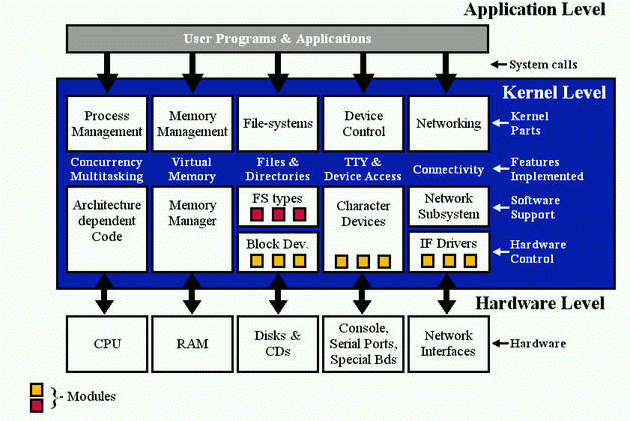
\includegraphics[width=10cm]{kernel_arch.png}
\end{frame}

\subsection{Système GNU/Linux}
\begin{frame}{Architecture}{Système GNU/Linux}
	Linux est un noyau. Seul il ne sert à rien. On parlera donc de système GNU/Linux.
	Il est en général composé de:
	\begin{itemize}
		\item
			Un bootloader (Rare sont les carte capable de booter un noyau Linux)\\
			Il est trop gros et doit etre chargé en RAM (elle doit etre initialisé par un microcode)
		\item
			Le noyau Linux (gérant les ressources de la machine)
		\item
			Un système de fichier contenant à minima un programme de démarrage (rootfs)
	\end{itemize}
\end{frame}

\subsection{Démarrage}
\begin{frame}{Architecture}{Démarrage}
	\begin{enumerate}
		\item
			Le matériel lance le bootloader
		\item
			Le bootloader configure la RAM et le support contenant le noyau 
		\item
			Le bootloader copie le noyau en RAM et lui donne la main
		\item
			Le noyau s'auto extrait en RAM
		\item
			Le noyau initialise les périphériques et les services (ordonnanceur, pile réseaux,syteme de fichier...)
		\item
			Le noyau récupère dans le rootfs le binaire d'initialisation (/sbin/init par défaut) et cré le processus 1
		\item
			Ce processus est chargé de démarrer tous les services en espaces utilisateurs.
	\end{enumerate}
\end{frame}

\subsection{Organisation d'un rootfs}
\begin{frame}{Architecture}{Organisation d'un rootfs}
	Organisation commune à 90% entre les UNIX
	Quelques spécificités GNU/Linux et distribution
	Les fichiers communs:
	\begin{itemize}
		\item
			/bin: binaires communs
		\item
			/lib: bibliothèques et modules noyau
		\item
			/sbin: binaires système
		\item
			/etc: fichiers de configuration
		\item
			/dev: nœuds d'accès aux périphériques (nodes)
		\item
			/var: fichiers variables: log, spool, mail, ...
		\item
			/usr: reproduit / pour bin, lib, sbin, etc
		\item
			/opt: pour les programmes externes (ex: OpenOffice)
		\item
			/home: accueille les répertoires des utilisateurs (home-directory)
	\end{itemize}
\end{frame}

\begin{frame}{Architecture}{Organisation d'un rootfs}	
	Quelques répertoires spéciaux:
	\begin{itemize}
		\item
			/root: home-directory de l'utilisateur root (pas dans OE)
		\item
			/media: point de montage des volumes amovibles
		\item
			/proc: système de fichier virtuel (état du système)
		\item
			/sys: idem pour les périphériques connectés (2.6)
		\item
			/boot: noyau statique (vmlinuz, uImage, ...)
	\end{itemize}
\end{frame}
